%%%%%%%%%%%%%%%%%%%%%%%%%%%%%%%%%%%%%%%%%%%%%%%%%%%%%%%%%%%%%%%%%%%%%%%%
\section{Problem 1: GANs on MNIST (40 points)}
%%%%%%%%%%%%%%%%%%%%%%%%%%%%%%%%%%%%%%%%%%%%%%%%%%%%%%%%%%%%%%%%%%%%%%%%
% Body below is gan-mnist-writeup.tex (hw3/hw3-update/), sections demoted one
% level, with the four sample grids added as figures.

\begin{question}
You will implement a Generative Adversarial Network model and evaluate it under different conditions, using the notebook \texttt{gan-mnist.ipynb}.
\begin{enumerate}
  \item[(a)] Part 1: Libraries and utility functions. Why do you think it is convenient to normalize the images to the range \([-1,1]\) instead of \([0,1]\)?
  (Bonus) How does the minimax game defined by the objective function of a GAN relate to minimizing the Jensen--Shannon divergence between the training data distribution and the samples obtained from the generator? (Bonus) Why is maximizing the probability of the discriminator making the INCORRECT choice the most practical way to update the generator?
  \item[(b)] Part 2: Vanilla GAN. Implement the noise sampling function as well as the generator and discriminator networks.
  \item[(c)] Part 3: GAN Loss. Implement the necessary losses for both networks.
  \item[(d)] Part 4: Training Function. Implement the optimizer construction, review and run the training loop cells. How do the generated samples look?
  \item[(e)] Part 5: Least Squares GAN. Implement the Least-Squares loss function and evaluate. How do the resulting generated samples compare to those produced by the Vanilla GAN? Why do you think this is the case?
  \item[(f)] Part 6: Deeply Convolutional GANs. Implement the generator and discriminator architectures and evaluate the resulting model. How do the generated samples compare to the two previous configurations? Why does adding convolutional layers have this effect?
  \item[(g)] Part 7: Compare generated images. Evaluate the generated samples from the three previous models against the real MNIST images. Can you distinguish the original from the fake ones in all three cases? Do you think an equilibrium exists where the generator wins, i.e.\ the discriminator ends up unable to distinguish the two distributions on finite samples? Explain why you believe this would or would not be possible.
\end{enumerate}
\end{question}

\subsection{Part 1: Libraries and Utility Functions}

The notebook defines the GAN as the minimax game
\begin{equation}
  \min_G \max_D \;
  \mathbb{E}_{x \sim p_{\mathrm{data}}}\!\left[\log D(x)\right]
  + \mathbb{E}_{z \sim p(z)}\!\left[\log \bigl(1 - D(G(z))\bigr)\right],
  \label{eq:minimax}
\end{equation}
and then replaces the generator step with
\begin{equation}
  \max_G \; \mathbb{E}_{z \sim p(z)}\!\left[\log D(G(z))\right].
  \label{eq:nonsat}
\end{equation}
\texttt{preprocess\_img} maps real images from \([0,1]\) to \([-1,1]\) by \(x \mapsto 2x-1\), and \texttt{deprocess\_img} maps them back for display.

\subsubsection{Normalization to \([-1,1]\)}

Scaling to \([-1,1]\) matches the generator's final \(\tanh\), whose outputs lie in \((-1,1)\). Real and generated images then share one scale, so the discriminator compares like with like and every real pixel value is one the generator can actually produce. The interval is also symmetric about zero, which keeps the inputs to both networks roughly zero-mean, and it matches the range of the latent noise.

\subsubsection{Minimax training and Jensen--Shannon divergence}

For a fixed generator, the discriminator that maximizes~\eqref{eq:minimax} is
\begin{equation}
  D_G^*(x) = \frac{p_{\mathrm{data}}(x)}{p_{\mathrm{data}}(x) + p_g(x)}.
\end{equation}
Substituting \(D_G^*\) back in gives
\begin{align}
  C(G)
  &= -\log 4
    + \mathrm{KL}\!\left(p_{\mathrm{data}} \middle\| \frac{p_{\mathrm{data}}+p_g}{2}\right)
    + \mathrm{KL}\!\left(p_g \middle\| \frac{p_{\mathrm{data}}+p_g}{2}\right) \nonumber \\
  &= -\log 4 + 2\,\mathrm{JSD}(p_{\mathrm{data}} \| p_g).
  \label{eq:jsd}
\end{align}
The inner maximization turns the game into a constant plus twice the Jensen--Shannon divergence between the data and generator distributions, so minimizing over \(G\) minimizes that divergence. The minimum, \(-\log 4\), is reached only when \(p_g = p_{\mathrm{data}}\), where \(D_G^*(x) = 1/2\) everywhere.

\subsubsection{Generator update}

Early in training the generator is weak and \(D(G(z)) \approx 0\). With \(D = \sigma(s)\) for a logit \(s\), the minimax generator term \(\log(1-D(G(z)))\) has gradient \(-D(G(z))\) with respect to \(s\), which goes to zero there, so the generator gets almost no signal.

The non-saturating update~\eqref{eq:nonsat} instead minimizes \(-\mathbb{E}_z[\log D(G(z))]\), whose gradient with respect to \(s\) is \(-(1 - D(G(z)))\). That is largest exactly when \(D(G(z))\) is near \(0\). It maximizes the probability that the discriminator is wrong on generated data, keeps the same fixed point (\(p_g = p_{\mathrm{data}}\), \(D = 1/2\)), and gives much larger gradients early on. The discriminator still trains on~\eqref{eq:minimax}.

\subsection{Part 2: Vanilla GAN}

\subsubsection{Noise sampling}

\texttt{sample\_noise(batch\_size, dim)} draws \texttt{torch.rand} of shape \((\texttt{batch\_size}, \texttt{dim})\), uniform on \([0,1]\), and maps \(u \mapsto 2u-1\). The result is the uniform prior on \([-1,1]\).

\subsubsection{Discriminator}

A fully connected classifier with biases and LeakyReLU slope \(0.01\):
\begin{center}
\begin{tabular}{lll}
\toprule
Layer & Shape & Activation \\
\midrule
Flatten & image \(\to\) \(784\) & none \\
Linear & \(784 \to 256\) & LeakyReLU(\(0.01\)) \\
Linear & \(256 \to 256\) & LeakyReLU(\(0.01\)) \\
Linear & \(256 \to 1\) & none \\
\bottomrule
\end{tabular}
\end{center}
It outputs one logit per image, shape \([\texttt{batch\_size}, 1]\). There is no sigmoid, so the loss can use a numerically stable cross-entropy on logits. The network has \(267{,}009\) parameters.

\subsubsection{Generator}

\begin{center}
\begin{tabular}{lll}
\toprule
Layer & Shape & Activation \\
\midrule
Linear & \(\texttt{noise\_dim} \to 1024\) & ReLU \\
Linear & \(1024 \to 1024\) & ReLU \\
Linear & \(1024 \to 784\) & \(\tanh\) \\
\bottomrule
\end{tabular}
\end{center}
The final \(\tanh\) puts every pixel in \((-1,1)\), the range of the preprocessed real images. With \(\texttt{noise\_dim} = 4\), as in the notebook's parameter check, the network has \(1{,}858{,}320\) parameters; training uses \(\texttt{NOISE\_DIM} = 96\).

\subsection{Part 3: GAN Loss}

Both losses are minibatch means of the provided stable binary cross-entropy on logits,
\[
  bce(s, y) = -y \log \sigma(s) - (1-y)\log\bigl(1-\sigma(s)\bigr),
\]
with real targets \(1\) and fake targets \(0\). Scores of shape \([N, 1]\) are flattened to length \(N\) so they line up with the labels, which are cast to the scores' device with \texttt{.type(dtype)}.

\subsubsection{Discriminator}

\[
  \ell_D
  = -\mathbb{E}_{x \sim p_{\mathrm{data}}}\!\left[\log D(x)\right]
  - \mathbb{E}_{z \sim p(z)}\!\left[\log \bigl(1 - D(G(z))\bigr)\right].
\]
In code this is \texttt{loss\_real + loss\_fake}: real logits against ones plus fake logits against zeros. Since \texttt{bce\_loss} returns a mean, the sum matches the two expectations. Minimizing it raises \(D(x)\) on real images and lowers \(D(G(z))\) on fakes.

\subsubsection{Generator}

The non-saturating objective from Part~1, written for minimization:
\[
  \ell_G = -\mathbb{E}_{z \sim p(z)}\!\left[\log D(G(z))\right].
\]
It is the cross-entropy between fake logits and ones, which pushes \(D(G(z))\) toward \(1\).

\subsection{Part 4: Training}

\subsubsection{Optimizer}

\texttt{get\_optimizer} returns Adam with learning rate \(10^{-3}\) and betas \((0.5, 0.999)\), used for every network in the notebook. \(\beta_1 = 0.5\) is the usual GAN choice: a shorter gradient memory suits a discriminator that keeps moving.

\subsubsection{Training loop}

The loop is provided. Each epoch runs the \(390\) full minibatches of \(128\) from the \(50{,}000\) training images (the incomplete last batch is skipped), for \(10\) epochs. Each iteration takes one discriminator step, then one generator step. Real images are scaled by \(2(x - 1/2)\), the same map as \texttt{preprocess\_img}. The discriminator step detaches the generated images, so only \(D\) is updated. The generator step draws fresh noise and scores the fakes with the updated \(D\); the gradients this leaves on \(D\) are cleared by the next iteration's \texttt{zero\_grad}. Every \(250\) iterations a fixed noise batch, drawn once at the start, is passed through \(G\) and saved to \texttt{v\_gan/image\_*.png}, so the same latent codes can be followed through training.

\subsubsection{Generated samples}

At iteration \(0\) every tile is gray pixel noise. By iteration \(250\) the mass has collapsed into bright, fuzzy blobs on a still-gray background, most with the same rough 8-like shape. By iteration \(1000\) the backgrounds are dark and the blobs have become soft digits: nines, sevens, zeros, and ones are recognizable, with speckled edges. At iterations \(3000\) and \(3750\) about half of the fixed seeds are clearly a digit (\(1\), \(4\), \(6\), \(7\)); the rest are broken or noisy, and speckle remains around most strokes. The discriminator loss stays near \(1.0\)--\(1.4\), around the equilibrium value \(2\log 2 \approx 1.39\), and the generator loss settles near \(0.8\)--\(1.1\) after an early spike. The samples cover a spread of digit classes rather than a single mode.

\begin{figure}[H]
  \centering
  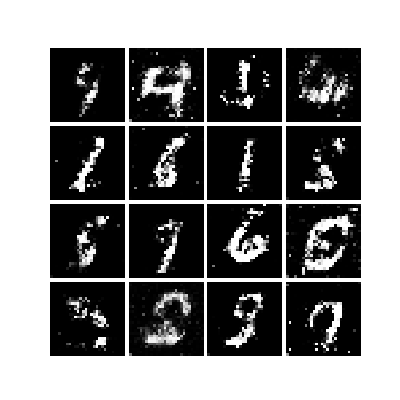
\includegraphics[width=0.55\linewidth]{v_gan/image_015.png}
  \caption{Vanilla GAN, this run's fixed latent codes at iteration 3750.}
  \label{fig:vgan}
\end{figure}

\subsection{Part 5: Least Squares GAN}

The networks and training loop stay the same; only the losses change, to equation~(9) of Mao et al.:
\begin{align}
  \ell_D
  &= \tfrac12 \mathbb{E}_{x \sim p_{\mathrm{data}}}\!\left[\bigl(D(x)-1\bigr)^2\right]
   + \tfrac12 \mathbb{E}_{z \sim p(z)}\!\left[\bigl(D(G(z))\bigr)^2\right], \\
  \ell_G
  &= \tfrac12 \mathbb{E}_{z \sim p(z)}\!\left[\bigl(D(G(z))-1\bigr)^2\right].
\end{align}
Each expectation is a minibatch mean of the raw scores. Against \texttt{gan-checks.npz} the errors are \(1.53\times 10^{-8}\) for the discriminator and \(2.78\times 10^{-9}\) for the generator, both under the \(10^{-7}\) tolerance.

\subsubsection{Comparison with the vanilla GAN}

At iteration \(1000\) the LS samples are still clusters of salt-and-pepper pixels, behind the vanilla grid at the same point. By iterations \(3000\) and \(3750\) most fixed seeds are a recognizable digit (\(5\), \(3\), \(9\), \(1\), \(4\), \(6\), \(7\)), with thicker and more complete strokes than the vanilla samples, where only about half are clearly digits. The gain is modest in this run: the speckle around the strokes is about as heavy as in the vanilla grid, a few seeds are still blobs, and the \(4\) repeats several times.

The more complete strokes come from the loss. The vanilla generator's cross-entropy saturates once a fake is on the real side of the decision boundary, so there is little gradient left to fix speckle or broken strokes. The LS generator loss has gradient proportional to \(D(G(z))-1\), which stays large until the score actually reaches \(1\), so fakes that already fool the classifier are still pulled toward the real data. With labels satisfying \(b-c=1\) and \(b-a=2\), Mao et al.\ show that the LS objective minimizes a Pearson \(\chi^2\) divergence. The \(0/1\) labels used here do not meet that condition, but the gradient argument still holds.

\begin{figure}[H]
  \centering
  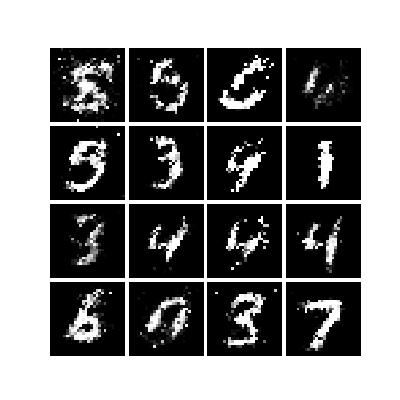
\includegraphics[width=0.55\linewidth]{ls_gan/image_015.png}
  \caption{LSGAN, this run's fixed latent codes at iteration 3750.}
  \label{fig:lsgan}
\end{figure}

\subsection{Part 6: Deep Convolutional GAN}

The loss is back to binary cross-entropy; the networks change. The discriminator unflattens to \(1\times 28\times 28\), then applies conv \(1\to 32\) (\(5\times 5\)), LeakyReLU(\(0.01\)), \(2\times 2\) max-pool, conv \(32\to 64\) (\(5\times 5\)), LeakyReLU, max-pool, flatten, linear \(1024\to 1024\), LeakyReLU, and linear \(1024\to 1\). It has \(1{,}102{,}721\) parameters and outputs shape \([128, 1]\).

The generator follows the InfoGAN layout: linear to \(1024\), ReLU, batch norm; linear to \(128\cdot 7\cdot 7\), ReLU, batch norm; reshape to \(128\times 7\times 7\); then two transposed convolutions (\(4\times 4\), stride \(2\), padding \(1\)) up to \(64\times 14\times 14\) and \(1\times 28\times 28\), with ReLU and batch norm between them and \(\tanh\) at the end. A final flatten returns a \(784\)-vector for the existing training loop. With \(\texttt{noise\_dim}=4\) it has \(6{,}580{,}801\) parameters. Xavier initialization is applied to every linear and transposed-convolution weight in both networks before training.

\subsubsection{Comparison with the fully connected GANs}

Iteration \(0\) is noise. By iteration \(1000\) the fixed seeds are already clean digits on a black background, ahead of where either fully connected model was at iteration \(3750\). At iteration \(3750\) the strokes are smooth and the backgrounds clean: \(1, 3, 7, 9, 8, 5, 8, 3, 1, 1, 5, 0, 9, 6, 7, 3\). A few tiles are slightly soft and the \(6\) is a bit malformed, but there is almost none of the salt-and-pepper noise in the vanilla and LS grids.

Convolution is the reason. A fully connected generator treats the \(784\) pixels as one vector, so nothing in its wiring says strokes are local or that the same edge can appear anywhere; the samples show that as speckle and broken contours. A convolutional discriminator looks at local patches with shared filters, so it judges stroke shape rather than a bag of pixels. The transposed convolutions build the image by upsampling a \(7\times 7\) spatial code, so neighboring pixels are produced together, and batch norm keeps the deeper generator stable. The result is coherent strokes much earlier in training.

The losses are less flattering than the images. Over the last \(1000\) iterations the discriminator loss sits near \(1.0\)--\(1.1\) and the generator loss near \(0.9\)--\(1.3\), on either side of the chance-level pair \(2\log 2 \approx 1.39\) and \(\log 2 \approx 0.69\), so the discriminator still separates real from fake better than chance.

\begin{figure}[H]
  \centering
  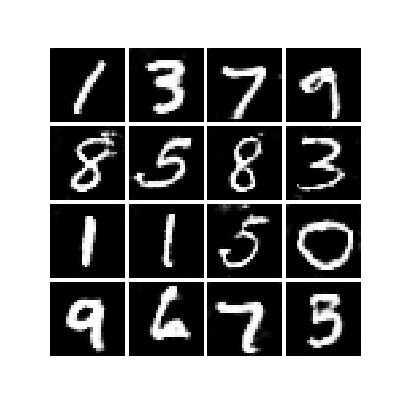
\includegraphics[width=0.55\linewidth]{dc_gan/image_015.png}
  \caption{DCGAN, this run's fixed latent codes at iteration 3750.}
  \label{fig:dcgan}
\end{figure}

\subsection{Part 7: Comparison with real MNIST}

Stacked against real digits, the three generators separate cleanly. Vanilla samples are easy to pick out: broken strokes, speckled backgrounds, and only about half are sharp digits. LS samples are only slightly harder; most are recognizable, but the strokes stay gritty and speckled. DCGAN samples are the close call, and many would pass as MNIST on their own. In a grid of \(50\) fakes over \(50\) reals (Figure~\ref{fig:realfake}), the real half is slightly crisper and the fake half still has the occasional stray pixel, soft edge, or slightly wrong stroke. That is enough to tell the two blocks apart, but not to label every single DCGAN image with confidence.

\begin{figure}[H]
  \centering
  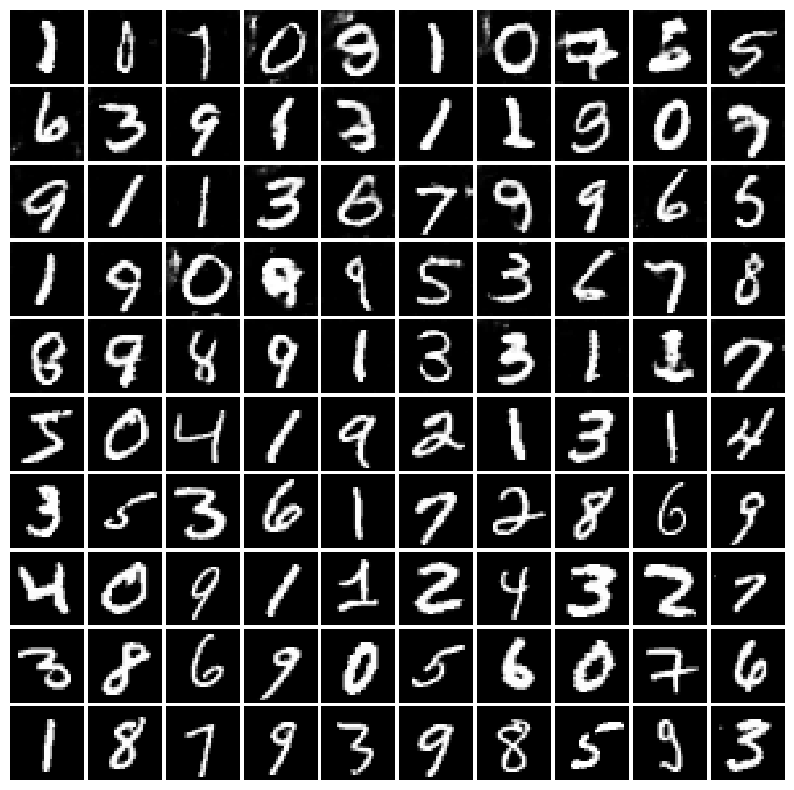
\includegraphics[width=0.85\linewidth]{dc_gan/real_vs_fake.png}
  \caption{DCGAN samples (top five rows) above real MNIST digits (bottom five rows).}
  \label{fig:realfake}
\end{figure}

\subsubsection{Can the generator win on finite samples?}

The game has an equilibrium, and it is a tie. Goodfellow et al.\ show that the optimal discriminator is \(D = 1/2\) everywhere exactly when \(p_g = p_{\mathrm{data}}\), with game value \(-\log 4\). The generator never ``wins'' by making the discriminator wrong; it can only match the data distribution, after which the discriminator's best strategy is to guess. This run does not reach that point even in the loss: the late DCGAN discriminator loss is about \(1.0\)--\(1.1\), not \(1.39\), so the discriminator being trained still separates real from fake on its minibatches.

Reaching chance in the training loss would still not make the two finite samples indistinguishable. A fresh, high-capacity classifier trained to convergence against a frozen generator can exploit any residual difference: speckle, a broken stroke, a small shift in stroke thickness. Making the two empirical distributions identical would require the generator to reproduce the training set, which none of these runs does. Vanilla and LS samples are obvious fakes, and DCGAN samples, though close, are still separable both by the training discriminator and by eye. So the equilibrium exists in theory, but a generator that makes finite samples truly indistinguishable is not something this run reaches, and it is not what one-step alternating updates on finite networks are set up to guarantee.
